\documentclass{article}
\usepackage{enumerate}
\usepackage{amsmath}
\usepackage{amssymb}
\usepackage{graphicx}
\usepackage{subfigure}
\usepackage{geometry}
\usepackage{caption}
\usepackage{indentfirst}
\usepackage{minted}
\usemintedstyle{autumn}
\setminted{linenos,breaklines,tabsize=4,xleftmargin=1.5em}
\geometry{left=3.0cm,right=3.0cm,top=3.0cm,bottom=4.0cm}
\renewcommand{\thesection}{Ex. \arabic{section} ---}
\newcommand{\unit}[1]{{\rm\,#1}}
\title{VE482 Homework 2}
\author{Liu Yihao 515370910207}
\date{}

\begin{document}
\maketitle

\section{Multiprogramming}
\begin{enumerate}
\item
The probability for $n$ processes to be waiting at the same time is $p^n$.\\
The CPU utilisation is $1-p^n$.
\item \
\begin{center}
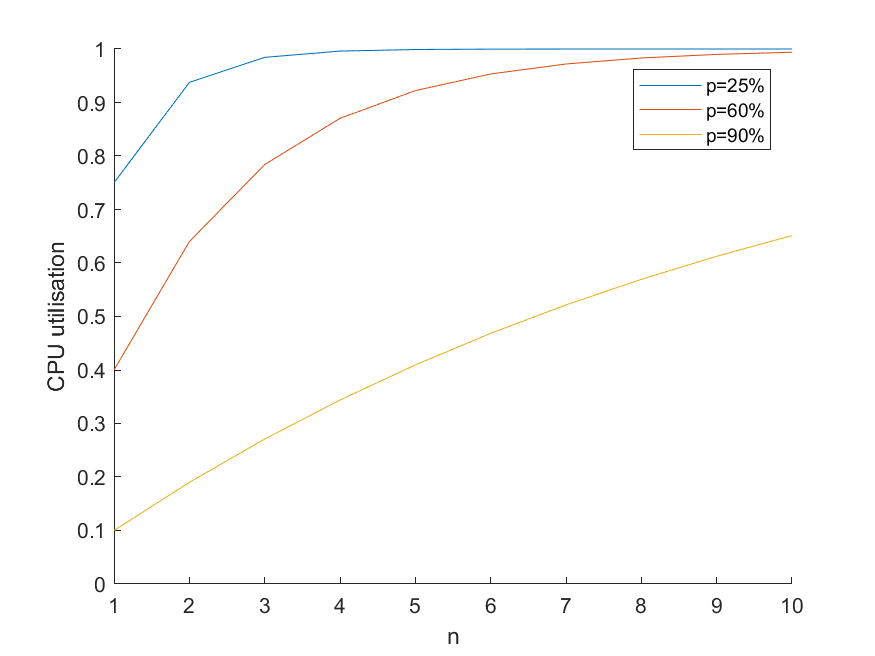
\includegraphics[width=0.8\linewidth]{ex1.png}
\end{center}
\item
\begin{enumerate}[a)]
\item
$$\lfloor(256-96)\div48\rfloor=3$$
So three processes can be store simultaneously in memory.
\item
$$1-0.9^3=27.1\%$$
So the CPU utilisation is $27.1\%$.
\item
When 256 MB is added, $\lfloor(512-96)\div48\rfloor=8$ processes can be store simultaneously in memory, the CPU utilisation is $1-0.9^8\approx56.95\%$. It has a improvement of $29.85\%$ per 256 MB.

When 512 MB is added, $\lfloor(768-96)\div48\rfloor=14$ processes can be store simultaneously in memory, the CPU utilisation is $1-0.9^8\approx77.12\%$. It has a improvement of $10.09\%$ per 256 MB.

When 1024 MB is added, $\lfloor(1280-96)\div48\rfloor=24$ processes can be store simultaneously in memory, the CPU utilisation is $1-0.9^8\approx98.02\%$. It has a improvement of $5.23\%$ per 256 MB.

In conclusion, we can find that adding the first 256 MB is the most beneficial and be worth the investment.

\end{enumerate}
\end{enumerate}

\section{Keymap in Minix 3}
There are three files to be modified.\\

The first file is \mintinline{shell}{minix/servers/is/dmp.c}

\begin{minted}{c}
struct hook_entry {
    int key;
    void (*function)(void);
    char *name;
} hooks[] = {
    { F1,   proctab_dmp, "Kernel process table" },
    { F3,   image_dmp, "System image" },
    { F4,   privileges_dmp, "Process privileges" },
    { F5,   monparams_dmp, "Boot monitor parameters" },
    { F6,   irqtab_dmp, "IRQ hooks and policies" },
    { F7,   kmessages_dmp, "Kernel messages" },
    { F8,   vm_dmp, "VM status and process maps" },
    { F10,  kenv_dmp, "Kernel parameters" },
    { SF1,  mproc_dmp, "Process manager process table" },
    { SF2,  sigaction_dmp, "Signals" },
    { SF3,  fproc_dmp, "Filesystem process table" },
    { SF4,  dtab_dmp, "Device/Driver mapping" },
    { SF5,  mapping_dmp, "Print key mappings" },
    { SF6,  rproc_dmp, "Reincarnation server process table" },
    { SF7,  proc_num_dmp, "Display the number of currently running processes" },
    { SF8,  data_store_dmp, "Data store contents" },
    { SF9,  procstack_dmp, "Processes with stack traces" },
};
\end{minted}

SF7 is added in order to map Shift + F7.\\

The second file is \mintinline{shell}{minix/servers/is/proto.h}
\begin{minted}{c}
/* dmp_kernel.c */
void proc_num_dmp(void); // Added by myself
void proctab_dmp(void);
void procstack_dmp(void);
void privileges_dmp(void);
void image_dmp(void);
void irqtab_dmp(void);
void kmessages_dmp(void);
void monparams_dmp(void);
void kenv_dmp(void);
\end{minted}

I added the definition of function \mintinline{c}{void proc_num_dmp(void)} here.\\

The third file is \mintinline{shell}{minix/servers/is/dmp_kernel.c}
\begin{minted}{c}
// Added by myself
/*===========================================================================*
 *                                proc_num_dmp                               *
 *===========================================================================*/
void proc_num_dmp(void)
{
    register struct proc *rp;
    int r;

    /* First obtain a fresh copy of the current process table. */
    if ((r = sys_getproctab(proc)) != OK) {
        printf("IS: warning: couldn't get copy of process table: %d\n", r);
        return;
    }

    int num = 0;
    for (rp = BEG_PROC_ADDR; rp < END_PROC_ADDR; rp++) {
        if (isemptyp(rp)) continue;
        num++;
    }
    printf("The number of currently running process is %d\n", num);
}
\end{minted}

I added the implementation of function \mintinline{c}{void proc_num_dmp(void)} here.\\

Then I build the kernal and test it.
\begin{minted}[breakanywhere]{shell}
./releasetools/x86_hdiimage.sh
cd ../obj.i386/destdir.i386/boot/minix/.temp && qemu-system-i386 -serial stdio -kernel kernel -append "rootdevname=c0d0p1" -initrd "mod01_ds,mod02_rs,mod03_pm,mod04_sched,mod05_vfs,mod06_memory,mod07_tty,mod08_mfs,mod09_vm,mod10_pfs,mod11_init" -hda ~/minix/minix-3.3.0/minix-3.3.0/minix_x86.img --enable-kvm
\end{minted}

\end{document}
